% Section content template for individual Educative lessons
% This file contains the actual content for a specific section
% Generated from Educative API section content

% Section: Introduction to Code Deployment System
% Section ID: 6349756689154048
% Section Slug: introduction-to-code-deployment-system
% Generated: 2025-12-08T15:26:19.345558

\subsection{What is a code deployment system?}\label{ikoZrLyWkbOl6Z9nbYt8f}
\\
A code deployment system is a set of processes, tools, and techniques, often referred to as a \textbf{deployment pipeline} or \textbf{continuous deployment system}. It automates the distribution and deployment of software code across various environments, including testing, staging(A staging environment is a controlled environment that closely mimics the production environment. It is used to test and validate code changes, new features, updates, and configurations before they are deployed to the production environment where end-users will access them. ), and production environments. Its main objective is to ensure that new code (or code changes) are smoothly and efficiently released from the development environment to the production environment while minimizing disruption and risk.
\\
This lesson introduces the fundamentals of code deployment. We 'll learn key steps in the deployment process, explore common deployment strategies, and understand how to estimate resources and requirements when designing a deployment system.

\subsubsection{Steps involved in the code deployment system}\label{foex7ljv6FDUsYM2eEp4G}
\\
A typical deployment system follows these key stages to move code from development to production:

\begin{enumerate}
\item
\protect\phantomsection\label{EUaWgMTFi2El2YKasrBjc}
\textbf{Version control:} Code deployment process begins with version control, where developers utilize a~\href{https://www.educative.io/courses/getting-started-with-git-version-control}{version control system}~(such as Git) to manage and track changes made to the codebase.
\item
\protect\phantomsection\label{D6HyS1o_TTqfEV7tgH3d7}
\textbf{Continuous integration (CI):} In a continuous integration phase, code changes from different developers are frequently integrated into a shared repository. Preliminary automated tests(These tests are designed to quickly identify issues in code changes, ensuring that new code additions or modifications do not introduce errors or defects. Preliminary automated tests help catch problems early in the development process, making it easier and less costly to fix them. ) are executed to ensure that the codebase remains stable and functional.
\item
\protect\phantomsection\label{SOA4aORUEgTXNrJrwPz2P}
\textbf{Build phase:} After successful integration, a build process is triggered. During this phase, the system compiles the code, resolves dependencies, and generates deployable artifacts or executable files (binaries).
\item
\protect\phantomsection\label{WKup23FeVwH09aZmJaXZj}
\textbf{Automated testing:~} The deployment system runs extensive automated tests to check for any regressions or defects that the changes may inadvertently introduce to existing features. Different automated testsAutomatedTests are performed in this phase depending on the organization's needs and the nature of the software.
\end{enumerate}

\subsection*{Quiz}
\vspace{0.3cm}
\noindent
\textbf{Question 1:} Question: How do automated tests in the deployment phase differ from those in CI?
\\[0.2cm]
\begin{itemize}
 \item Deployment tests run only on developer machines.
 \item CI tests are optional, but deployment tests are mandatory.
 \item \textbf{[CORRECT]} CI tests validate code changes early, while deployment tests validate the full system before release.
 \item CI tests focus on performance and load testing.
\end{itemize}

\begin{enumerate}
\setcounter{enumi}{4}
\item
\protect\phantomsection\label{TG6BBiOujXgxJQR1TRcPq}
\textbf{Staging environment:} The code changes are deployed to a staging environment that closely mimics the production environment. This enables additional testing and validation before the software is released to production.
\item
\protect\phantomsection\label{rOZ85eEUnftLkW1PqelU7}
\textbf{Deployment phase:} The code deployment system automatically deploys the tested and approved code changes to the production environment. This includes downloading code artifacts from the storage to each machine in the selected environment. This is often done gradually or using feature flags(Feature flags control whether or not an application's features or functionality are enabled or disabled. When we copy artifacts to our development environment, we can use feature flags to manage and control what features are turned on or off for testing and development.) to minimize the risk of potential issues.
\item
\protect\phantomsection\label{KZQAfdCi2HeuUFxOszAmt}
\textbf{Monitoring and rollback:} After deployment, the system continuously monitors the application's performance and user feedback. If any issues are detected, a rollback plan is in place to revert to the previous stable version.
\end{enumerate}

\begin{figure}[htbp]
 \centering
 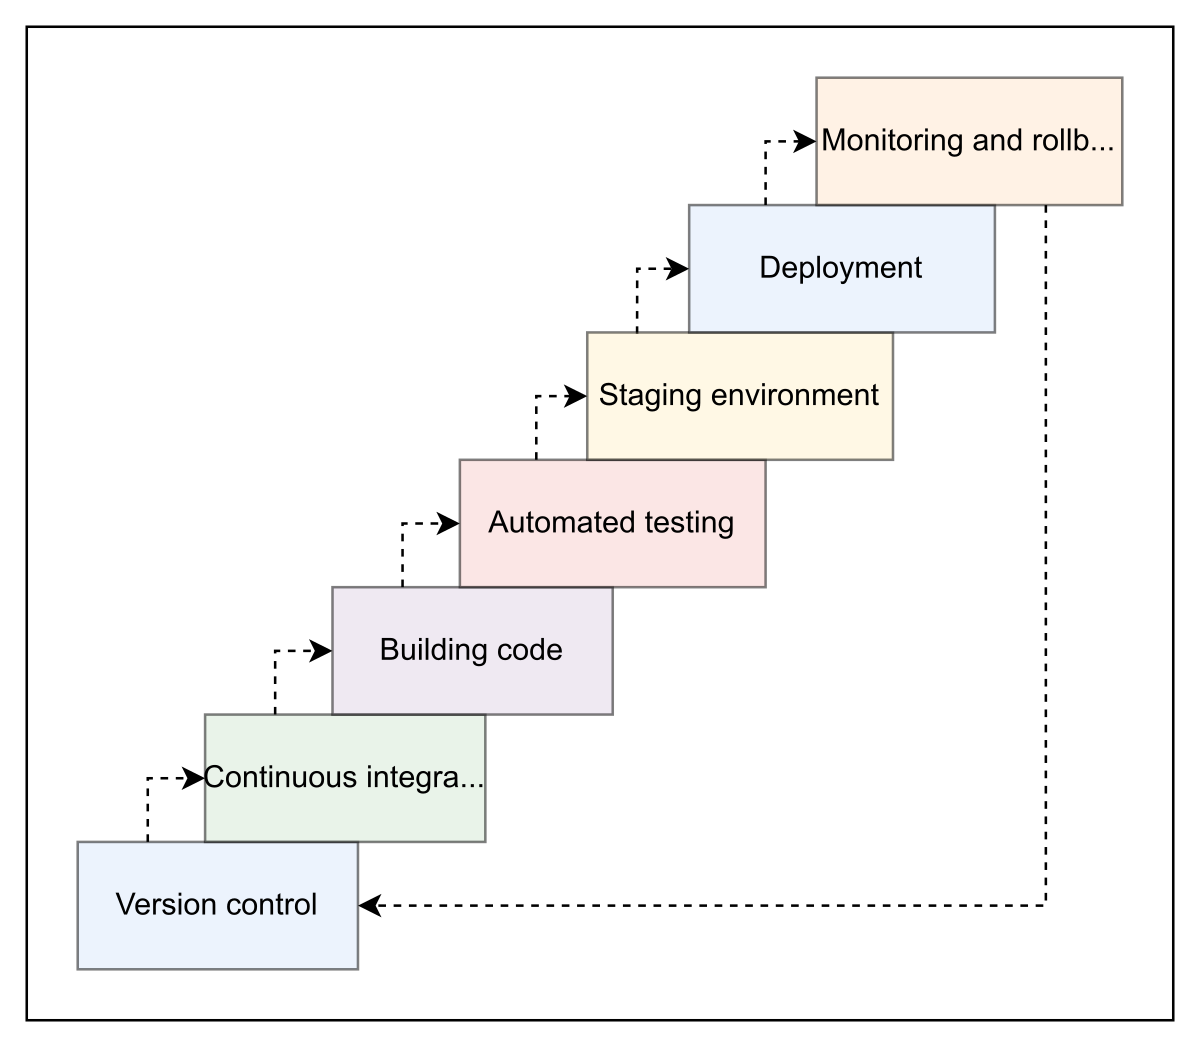
\includegraphics[width=0.5\textwidth]{Images/chapter_39/section_6349756689154048/4555759721250816.png}
 \caption{Steps involved in the code deployment system}
\end{figure}

Before designing the code deployment system, let's examine the various deployment strategies that influence the design.

\subsubsection{Code deployment strategies}\label{-nMew-2mx7wCjSIVpZ7bc}
\\
Code deployment strategies~are techniques used to release new code versions into production while minimizing downtime, risk, and user disruption. They define the approach to rolling out updates to users rather than the operational steps of building and deploying code. Below are several widely used strategies:

\begin{itemize}
\item
\protect\phantomsection\label{S7YRRTDgrRyPE-P0_I9zu}
\textbf{Basic deployment:} Basic deployment involves directly releasing new code changes to the production environment. While simple, this approach can be risky, as it provides no safety net or rollback mechanism in case issues arise. It's generally unsuitable for large-scale or critical systems where reliability is essential.
\end{itemize}

\begin{figure}[htbp]
 \centering
 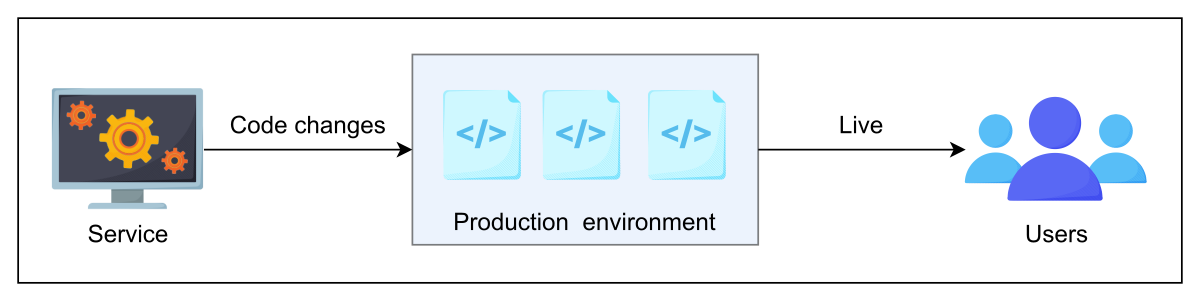
\includegraphics[width=0.5\textwidth]{Images/chapter_39/section_6349756689154048/6257248200163328.png}
 \caption{Releasing code directly to production}
\end{figure}

\begin{itemize}
\item
\protect\phantomsection\label{7NrJsFQwGJRcazYcnKhQj}
\textbf{Multi-service deployment:} In multi-service deployment, multiple interconnected services are updated simultaneously as part of a coordinated release. This strategy ensures consistency among related services and prevents compatibility issues arising from mismatched versions. While it supports cross-service(Cross-service changes in deployment refer to modifications or updates that affect multiple interconnected services within a software application.) changes, coordinating the release of multiple services can be complex.
\end{itemize}

\begin{figure}[htbp]
 \centering
 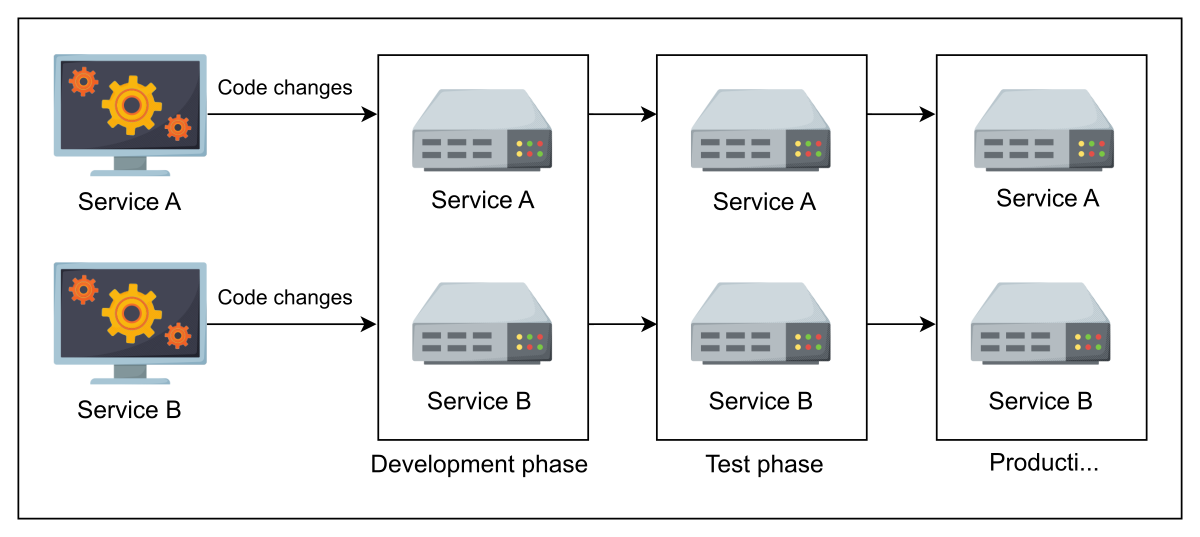
\includegraphics[width=0.5\textwidth]{Images/chapter_39/section_6349756689154048/5414674663079936.png}
 \caption{Releasing multiple dependent services together or in coordination to maintain system compatibility and stability}
\end{figure}

\begin{itemize}
\item
\protect\phantomsection\label{Ap0HCYXJVdEfexK0jb8V5}
\textbf{Rolling deployment:} Rolling deployment entails gradually deploying new code changes to a subset of servers while maintaining the current version on others. This minimizes downtime, ensures a gradual and controlled rollout, and distributes the load evenly across all services. However, slower than other strategies, they are straightforward to automate, which reduces the risk of widespread issues.
\end{itemize}

\begin{figure}[htbp]
 \centering
 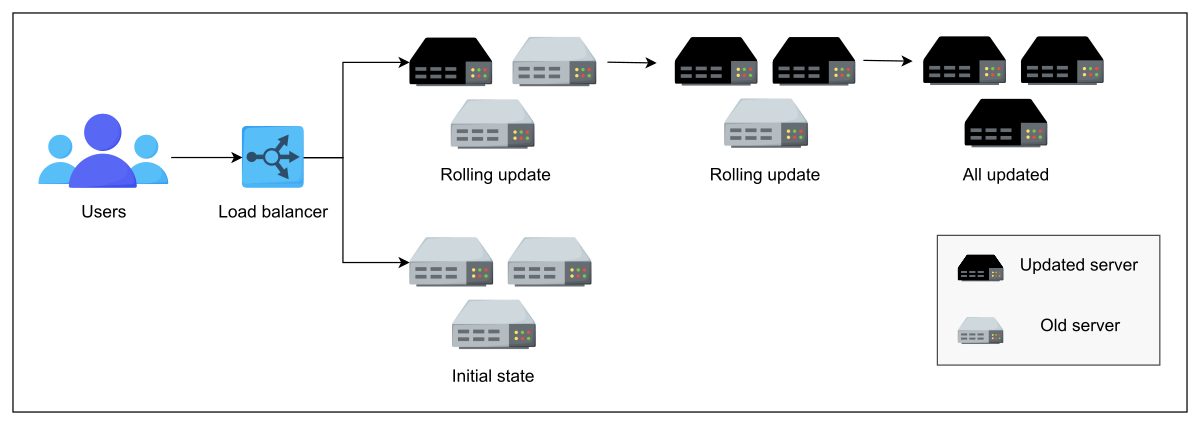
\includegraphics[width=0.5\textwidth]{Images/chapter_39/section_6349756689154048/5830668015501312.png}
 \caption{Updating servers in batches to avoid downtime}
\end{figure}

\begin{itemize}
\item
\protect\phantomsection\label{l8aqgw0RR2G_3jD80y-di}
\textbf{Blue-green deployment:} Blue-green deployment maintains two identical environments, one serving as the active production environment and the other for deploying new changes. This strategy offers minimal downtime, easy rollback, and a reduced risk of production issues. However, it requires duplicate infrastructure and introduces complexity in managing two separate environments.
\end{itemize}

\begin{figure}[htbp]
 \centering
 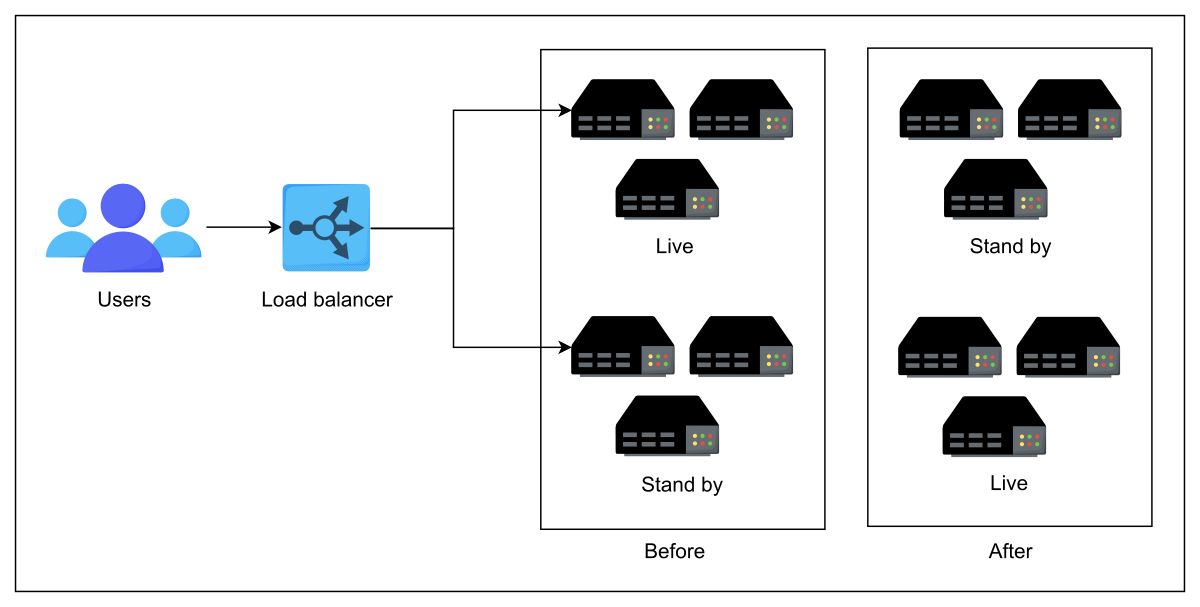
\includegraphics[width=0.25\textwidth]{Images/chapter_39/section_6349756689154048/6379754686906368.png}
 \caption{Switching traffic between two identical environments}
\end{figure}

\begin{itemize}
\item
\protect\phantomsection\label{Adm0gWKuyNk9i65R8Yerj}
\textbf{Canary deployment:} This approach releases new code changes to a small subset of servers and opens them to some users (canaries) before deploying them to the entire fleet. This approach enables early bug detection, gradual rollout, and limited issue impact. It requires monitoring to ensure that canary users have a positive experience, and it can be complex to manage with different user segments.
\end{itemize}

\begin{figure}[htbp]
 \centering
 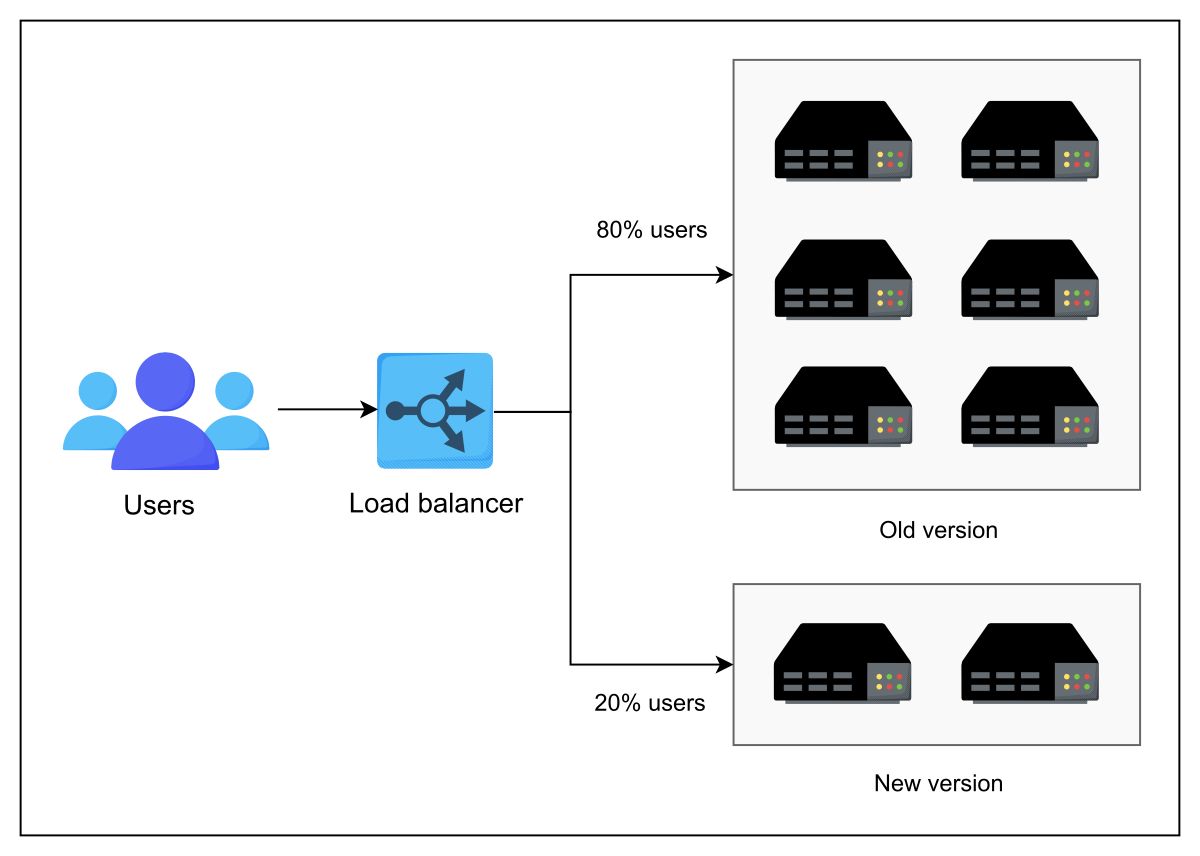
\includegraphics[width=0.25\textwidth]{Images/chapter_39/section_6349756689154048/6570380166561792.png}
 \caption{Gradually rolling out changes to a small group before full release}
\end{figure}

How would you decide which deployment strategy to use for a system that cannot afford any downtime?
\\
Use the AI assessment widget below to submit your solution and get an interactive response.

\textbf{Question:}

Deployment strategies

\textbf{Reference Answer:}

Strategies like blue-green or canary deployment are preferable because they allow updates without interrupting the live system and provide quick rollback options.

We have explored different code deployment strategies. Now , let's shift focus to designing a system that can support these strategies and execute the deployment sequence effectively.

\subsection{Requirements}\label{OX1aTHpDnMTVIq-FP2jEy}
\\
Below are the functional and non-functional requirements of a code deployment system.

\subsubsection{Functional requirements}\label{51OqBzNDLQLHuBIIjzZPT}
\\
Here are some essential functional requirements for a code deployment system:

\begin{itemize}
\item
\protect\phantomsection\label{xKq5-ugV19yVi4NlCFL3s}
\textbf{Building code:} The system should be able to build the code within a designated timeframe, for example, 20 minutes. The compilation process might generate a binary file of several gigabytes.
\item
\protect\phantomsection\label{ZzK2BpGxvD9cPGA4ZFV7y}
\textbf{Deploying code:} The system should be able to deploy code to many machines in several distinct worldwide regions.
\item
\protect\phantomsection\label{FMepc4G1LH_7nF2NGqs-l}
\textbf{Version control integration:} The system should be able to integrate with version control systems to fetch the latest code from repositories.
\item
\protect\phantomsection\label{Sx-cCGKfmaIedbnjBs2c-}
\textbf{Environment configuration:} It should allow users to define and manage environment-specific configurations, such as database connections, API endpoints, and other settings.
\item
\protect\phantomsection\label{-IV5vaxvs2sAM0xz4Rf7R}
\textbf{Rollback:} The system should facilitate the ability to roll back to previous code versions in case of issues.
\item
\protect\phantomsection\label{u1sq6AEJyv74v2tREje0c}
\textbf{Deployment monitoring:} It should provide monitoring and reporting features to track the progress and success of deployments.
\end{itemize}

\begin{figure}[htbp]
 \centering
 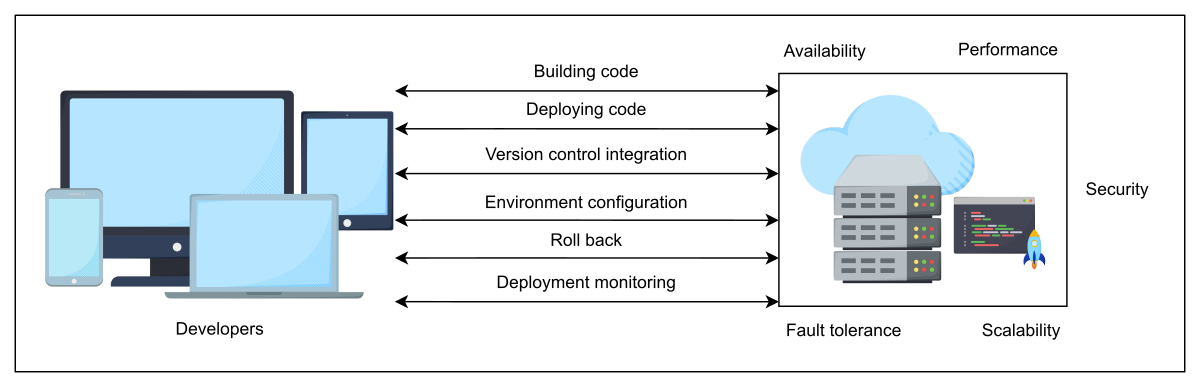
\includegraphics[width=0.5\textwidth]{Images/chapter_39/section_6349756689154048/4777121463271424.png}
 \caption{Functional and non-functional requirements of the code deployment system}
\end{figure}

\subsubsection{Non-functional requirements}\label{G53a5AVfkJBqWqz6qqfdW}
\\
The following are some non-functional requirements for a code deployment system:

\begin{itemize}
\item
\protect\phantomsection\label{PUTGcwf4BcYvgnoxrEWDk}
\textbf{Availability:} The code deployment system should strive for high availability to minimize downtime, incorporating redundancy, failover mechanisms, and zero-downtime deployment strategies to ensure maximum reliability.
\item
\protect\phantomsection\label{9sN9mwY0eE2hAjyo_hsSY}
\textbf{Fault tolerance:} Failures should be handled gracefully, with every build reaching \texttt{success} or \texttt{failure}.
\item
\protect\phantomsection\label{BsNc_5HTqWGCUH7sT2H90}
\textbf{Performance:} Deployments should start and finish within acceptable limits to minimize delays while meeting the required deployment rate.
\item
\protect\phantomsection\label{2zCHD-ion4gwcdR5SrPBE}
\textbf{Scalability:} The system should be able to handle increased load by scaling resources vertically or horizontally as required.
\item
\protect\phantomsection\label{MJh9dZXLCOPZcyShalW99}
\textbf{Security:} Sensitive data such as credentials and configuration data should be encrypted during transmission and storage. Similarly, every deployment action should be logged to maintain accountability.
\end{itemize}
\\
Why is managing environment-specific configurations critical for a deployment system?
\\
Use the AI assessment widget below to submit your solution and get an interactive response.

\textbf{Question:}

Requirements

\textbf{Reference Answer:}

Managing environment-specific configurations is essential because each environment--development, staging, and production--requires different settings for security, performance, and integrations; keeping them separate prevents failures, avoids accidental misuse of production resources, and ensures reliable, predictable deployments.

Now, we'll estimate the required resources for our system based on the requirements.

\subsection{Resource estimation}\label{cRli8oFxo0HIcWgiyLN2d}
\\
Assume that engineering teams across the globe deploy hundreds of services thousands of times each day. Each code build can take up to 20 minutes, generating numerous code artifacts. Based on this assumption, let's estimate the required resources in the following section:
\\
\textbf{Note:} The 20-minute timeframe is a general guideline and not a strict requirement. Actual build times may vary depending on factors such as the size and complexity of the codebase, the available build infrastructure (e.g., caching, distributed compilation, or build farms), and the nature of the application being built (e.g., embedded systems may require longer build times compared to web applications).

\subsubsection{Storage estimation}\label{GDigm1scJOGflejl-MHyw}

Let's estimate the amount of storage required based on the following assumptions:

\begin{itemize}
\item
\protect\phantomsection\label{PzmDKc3z94AuyeMZ4yk9p}
Number of applications (code updates): \protect\phantomsection\label{katex_inline_mNyJ3MLj642JKbvVdFFbf}{{{\(200 \)}}}
\item
\protect\phantomsection\label{0oSir6GsHjzdX-ZZ5rDwi}
Frequency of deployments: \protect\phantomsection\label{katex_inline_G9iUu27afZ_ptwZh_u9lW}{{{\(3000 \text{ per day}\)}}}
\item
\protect\phantomsection\label{yguo01SD8vkz7Vraqf53m}
Storage required for a single build: \protect\phantomsection\label{katex_inline_Q4h_uY2orPioEsgLQ-p9y}{{{\(20 \text{ GB}\)}}}
\item
\protect\phantomsection\label{LheP1au-KecktfeEtHJRx}
The total amount of storage required to store binaries per day for all applications (code updates):
\end{itemize}

\[
\text{Total storage}=\text{200}\times\text{3000}\times\text{20 GB = 12 PB}
\]

\begin{quote}
\textbf{Note:} This is a simplistic storage estimation based on deployment frequency and build size. In reality, factors like versioning, redundancy, backups, compression, and metadata could increase the required storage.
\end{quote}

The following calculator computes the total amount of storage required per day:

\subsubsection{Bandwidth estimation}\label{KCfWXh6y6NnQvVvx3dNxv}

A code build takes 20 minutes, followed by a 5-minute transfer to the regional blob store, considering network latency. With 2,000 machines per region, this 5-minute window is used to distribute the binaries across all machines. We can now estimate the required bandwidth to copy 20 GB binaries to each machine in 5 minutes, as follows:

\[
\text{Bandwidth = }\frac{\text{20 GB}}{\text{5 minutes}} \approx \text{533.3 Mbps}
\]


\subsubsection{The number of servers estimation}\label{9ldi01a2AAUpFA6Ts76cI}

To estimate the number of servers required, we consider the total number of deployments (3,000) per day. On average, a single server can perform up to 50 deployments per day. So , according to these numbers, the total number of servers required per day would be:

\begin{align*}
\text{Number of servers} &= \frac{\text{Total deployments (per day)}} {\text{Server's deployment capacity}} \\
&= \frac{3000}{50} \\
&= 60 \text{ servers}
\end{align*}

\begin{figure}[htbp]
 \centering
 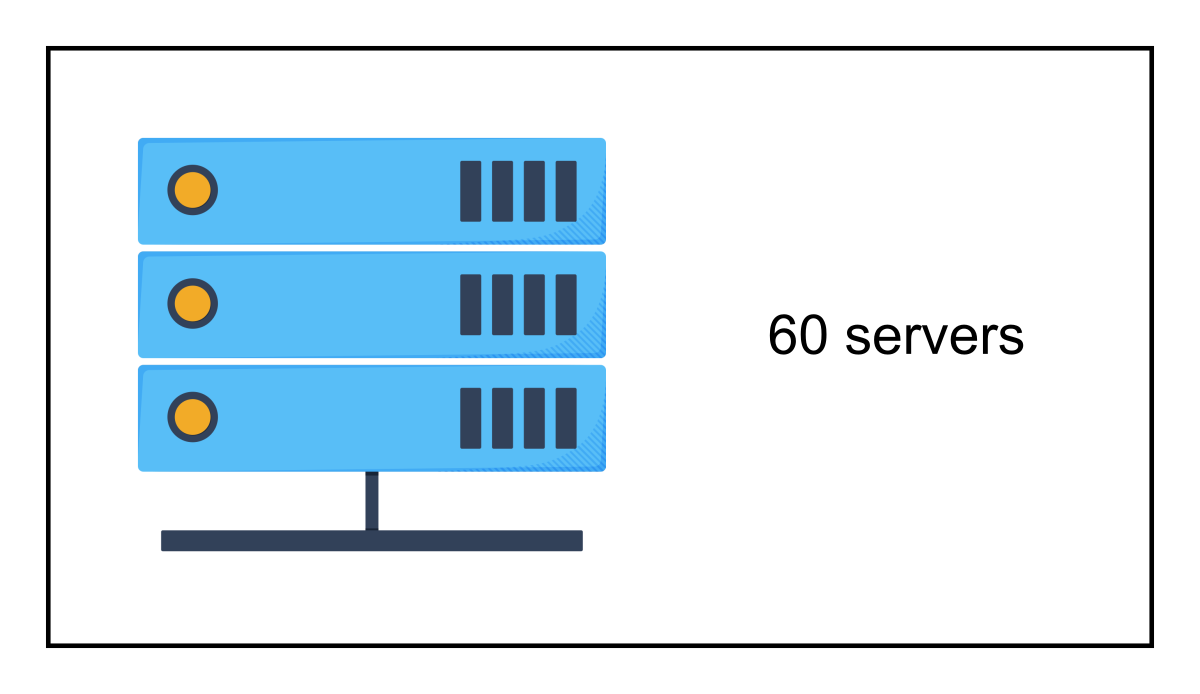
\includegraphics[width=0.25\textwidth]{Images/chapter_39/section_6349756689154048/5014272914358272.png}
 \caption{The number of servers required to perform 3000 deployments per day}
\end{figure}

\textbf{Note:}~These time estimates reflect typical scenarios and can vary based on factors such as codebase complexity, infrastructure (e.g., build farms, caching, parallelism), deployment scale (e.g., number of services), and application type (e.g., microservices vs. monoliths). Environmental conditions, such as network speed and deployment tool performance, may also affect timing.

\subsection{Building blocks we will use}\label{H0tfoPCL-O_Uxa-kugkDN}

The design of a code deployment system utilizes the following building blocks:

\begin{figure}[htbp]
 \centering
 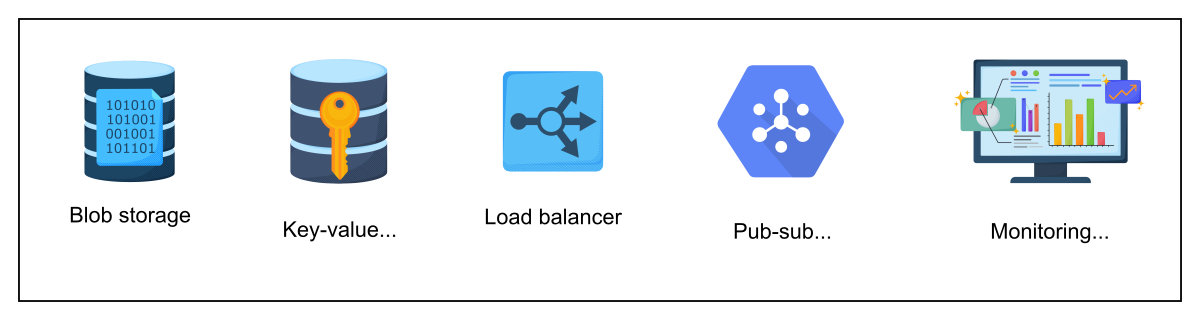
\includegraphics[width=0.5\textwidth]{Images/chapter_39/section_6349756689154048/4750071692132352.png}
 \caption{Building blocks required to design a code deployment system}
\end{figure}

\begin{itemize}
\item
\protect\phantomsection\label{Zrdy08HMRV991oSsAUdl1}
\href{https://www.educative.io/courses/grokking-the-system-design-interview/system-design-a-blob-store}{\textbf{Blob storage}} is necessary for storing code binaries (artifacts) during the code build and deployment phases.
\item
\protect\phantomsection\label{TkszB3K9bKo4C8PNp1StK}
\href{https://www.educative.io/courses/grokking-the-system-design-interview/system-design-the-key-value-store}{\textbf{Key-value stores}} are used to store the configuration information.
\item
\protect\phantomsection\label{oV3PipbIkM1fNRY3y1dVF}
\href{https://www.educative.io/courses/grokking-the-system-design-interview/introduction-to-load-balancers}{\textbf{Load balancers}} are used to distribute user requests among different servers and services.
\item
\protect\phantomsection\label{-NDoaSiK6V_GiHMiD8fCc}
\href{https://www.educative.io/courses/grokking-the-system-design-interview/system-design-the-pub-sub-abstraction}{\textbf{A pub-sub system}} is required to keep the code in the queue when the code build service is busy.
\item
\protect\phantomsection\label{S8Hjd4iIWwBPkPIzniwyj}
\href{https://www.educative.io/courses/grokking-the-system-design-interview/system-design-distributed-monitoring}{\textbf{A monitoring service}} checks the health of machines in the system.
\end{itemize}

In the next lesson, we'll focus on designing a code deployment system.

% End of section content